\documentclass{article}
\usepackage{GraphDefinitions}

\begin{document}

\begin{figure}[H]
\centering
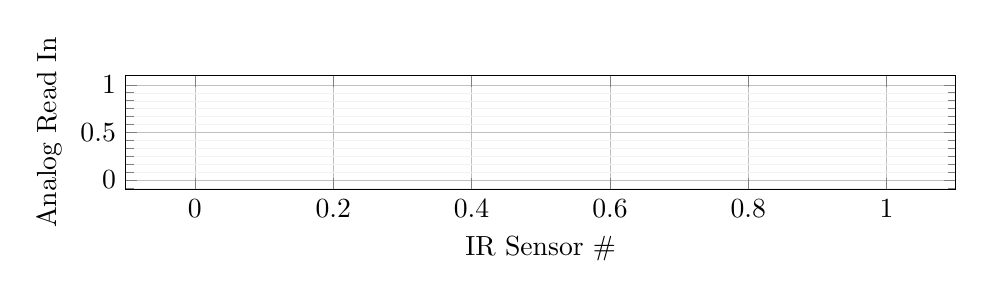
\begin{tikzpicture}
\begin{axis}[
    width=1\textwidth, % Adjust the width as needed
    height=0.25\textwidth, % Adjust the height as needed
    xlabel={IR Sensor \#},
    ylabel={Analog Read In},
    xtick={1, 2, 3, 4, 5, 6, 7}, % Set specific x-axis labels
    legend pos=north west,
    grid=both,
    grid style={line width=.1pt, draw=gray!10},
    major grid style={line width=.2pt,draw=gray!50},
    minor y tick num=5, % This adds the minor grid lines on the y-axis
    minor x tick num=0, % This removes the minor grid lines on the x-axis
    ]
    \IRTrace{green}{Green}{green}
    \IRTrace{blue}{Blue}{blue}
    \IRTrace{red}{Red}{red}
    \IRTrace{yellow}{Yellow}{black}
    \IRTrace{black}{Off}{black}
\end{axis}
\end{tikzpicture}
\caption{IR Calibration Data Based on Tape Color.}
\label{ir-calibration-data}
\end{figure}

\end{document}
